\documentclass{beamer}
\usepackage[utf8]{inputenc}
\usepackage[inline]{enumitem}
\usepackage{pdfpages}
\usepackage{listings}
\usepackage{subcaption}
\usepackage{wasysym}
\usepackage[export]{adjustbox}[2011/08/13]
\usetheme{cern}

\newcommand{\btVFill}{\vskip0pt plus 1filll}

% fix tilde
% \newcommand{\propertilde}{\raise.17ex\hbox{$\scriptstyle\mathtt{\sim}$}}

% \setbeameroption{show notes on second screen=right}

%The CERN logo is legally protected. Please visit http://cern.ch/copyright for
%information on the terms of use of CERN content, including the CERN logo.

% The optional `\author` command defines the author and is displayed in the
%slide produced by the `\titlepage` command.
\author{Corné Lukken \& Animesh Trivedi}

% The optional `\title` command defines the title and is displayed in the slide
%produced by the `\titlepage` command.
\title{OpenCSD: Log-Structured Filesystem enabled Computational Storage Device
platform}

% The optional `\subtitle` command will add a smaller title below the main one,
%and will not be displayed in any of the slides' footer.
% \subtitle{A SPDK compared to lightnvm story}

% The optional `\date` command will display a custom free text date on the all
%of the slides' footer. If omitted today's date will be used.
%\date{Monday, 1st January 2018}

% ------------------------------------------------------------------------%
% Proper Python Syntax Highlighting                                       %
% Author: redmode
% https://tex.stackexchange.com/questions/83882/how-to-highlight-python   %
% -syntax-in-latex-listings-lstinputlistings-command#83883                %
% ----------------------------------------------------------------------- %

% Default fixed font does not support bold face
\DeclareFixedFont{\ttb}{T1}{txtt}{bx}{n}{6} % for bold
\DeclareFixedFont{\ttm}{T1}{txtt}{m}{n}{6}  % for normal

% Custom colors
\definecolor{deepblue}{rgb}{0,0,0.5}
\definecolor{deepred}{rgb}{0.6,0,0}
\definecolor{deepgreen}{rgb}{0,0.5,0}

% Python style for highlighting
\newcommand\pythonstyle{
	\lstset{
		language=Python,
		basicstyle=\ttm,
		showstringspaces=false,
		tabsize=2,
		aboveskip=0.1cm,
		belowskip=0.1cm,
		otherkeywords={self},             % Add keywords here
		keywordstyle=\ttb\color{deepblue},
		emph={MyClass,__init__},          % Custom highlighting
		emphstyle=\ttb\color{deepred},    % Custom highlighting style
		stringstyle=\color{deepgreen},
		frame=tb,                          % Any extra options here
		prebreak=\textbackslash,
		linewidth=7.00cm,
		breaklines=true,
	}
}

% Python environment
\lstnewenvironment{python}[1][] {
	\pythonstyle\lstset{#1}
}{}

% Python for inline
\newcommand\pythoninline[1]{{\pythonstyle\lstinline!#1!}}

% Python for external file
\newcommand\pythonexternal[2][]{{\pythonstyle\lstinputlisting[#1]{#2}}}

\newcommand\pythonfullstyle{
	\lstset{
		language=Python,
		basicstyle=\ttm,
		showstringspaces=false,
		tabsize=2,
		aboveskip=0.1cm,
		belowskip=0.1cm,
		otherkeywords={self},             % Add keywords here
		keywordstyle=\ttb\color{deepblue},
		emph={MyClass,__init__},          % Custom highlighting
		emphstyle=\ttb\color{deepred},    % Custom highlighting style
		stringstyle=\color{deepgreen},
		frame=tb,                          % Any extra options here
		prebreak=\textbackslash,
		linewidth=11.00cm,
		breaklines=true,
	}
}

% Python environment
\lstnewenvironment{pythonfull}[1][] {
	\pythonfullstyle\lstset{#1}
}{}

% Python for inline
\newcommand\pythonfullinline[1]{{\pythonfullstyle\lstinline!#1!}}

% Python for external file
\newcommand\pythonfullexternal[2][]{{\pythonfullstyle\lstinputlisting[#1]{#2}}}

% ----------------------------------------------------------------------- %

% Bash style for highlighting
\newcommand\bashstyle{
	\lstset{
		language=Bash,
		basicstyle=\ttm,
		showstringspaces=false,
		tabsize=2,
		%commentstyle=itshape,
		aboveskip=0.1cm,
		belowskip=0.1cm,
		prebreak=\textbackslash,
		extendedchars=true,
		mathescape=false,
		% literate= {\$}{{\textcolor{blue}{\$}}}1 {&}{{\textcolor{blue}{\&}}}1 {/n}{{\textcolor{green}{\textbackslash n}}}1,
		linewidth=11cm,
		breaklines=true
	}
}

% Bash environment
\lstnewenvironment{bash}[1][] {
	\bashstyle\lstset{#1}
}{}

% Bash for inline
\newcommand\bashinline[1]{{\bashstyle\lstinline!#1!}}

% Bash for external file
\newcommand\bashexternal[2][]{{\bashstyle\lstinputlisting[#1]{#2}}}

% Python style for highlighting
\newcommand\cstyle{
	\lstset{
		language=c,
		basicstyle=\ttm,
		showstringspaces=false,
		tabsize=4,
		aboveskip=0.2cm,
		belowskip=0.2cm,
		otherkeywords={self},             % Add keywords here
		emph={MyClass,__init__},          % Custom highlighting
		keywordstyle=\ttb\color{deepblue},
		emphstyle=\ttb\color{deepred},    % Custom highlighting style
		stringstyle=\ttm\color{deepgreen},
%		identifierstyle=\ttm,
%		commentstyle=\ttm,
%		numberstyle=\ttm,
%		indexstyle=\ttm,
%		directivestyle=\ttm,
		frame=tb,                          % Any extra options here
		prebreak=\textbackslash,
		linewidth=5cm,
		breaklines=true,
	}
}

% Python environment
\lstnewenvironment{clist}[1][] {
	\cstyle\lstset{#1}
}{}

% Python for inline
\newcommand\cinline[1]{{\cstyle\lstinline!#1!}}

% Python for external file
\newcommand\cexternal[2][]{{\cstyle\lstinputlisting[#1]{#2}}}

\begin{document}

% page 1
\frame{\titlepage}
\begin{frame}{What is Computational Storage}
	\begingroup
	\small
	\begin{itemize}
		\item Bring compute closer to storage
		\item Numerous methods and architectures % compute element shared PCIe complex vs on device
		\item Different applications % Machine learning, key-value stores, transparent encryption
		\item Many benefits % Energy efficient, reduce host load, scalability
		\item Also many challenges % Mult-user tenancy and safety, filesystem integration, cumbersome APIs
		\item A long time in the making [1] % it has taken over a decade without any widespread adoption
	\end{itemize}
	\textit{\tiny $^{1}$Past, Present and Future of Computational Storage: A
	Survey, Corne Lukken \& Animesh Trivedi - https://arxiv.org/abs/2112.09691}
	\endgroup
\end{frame}

% page 2
\begin{frame}{Why Computational Storage}
	\begingroup
	\small
	% Where do the benefits come from; von nuemann, bandwidth bottlenecks
	\begin{figure}
	   \centering
	   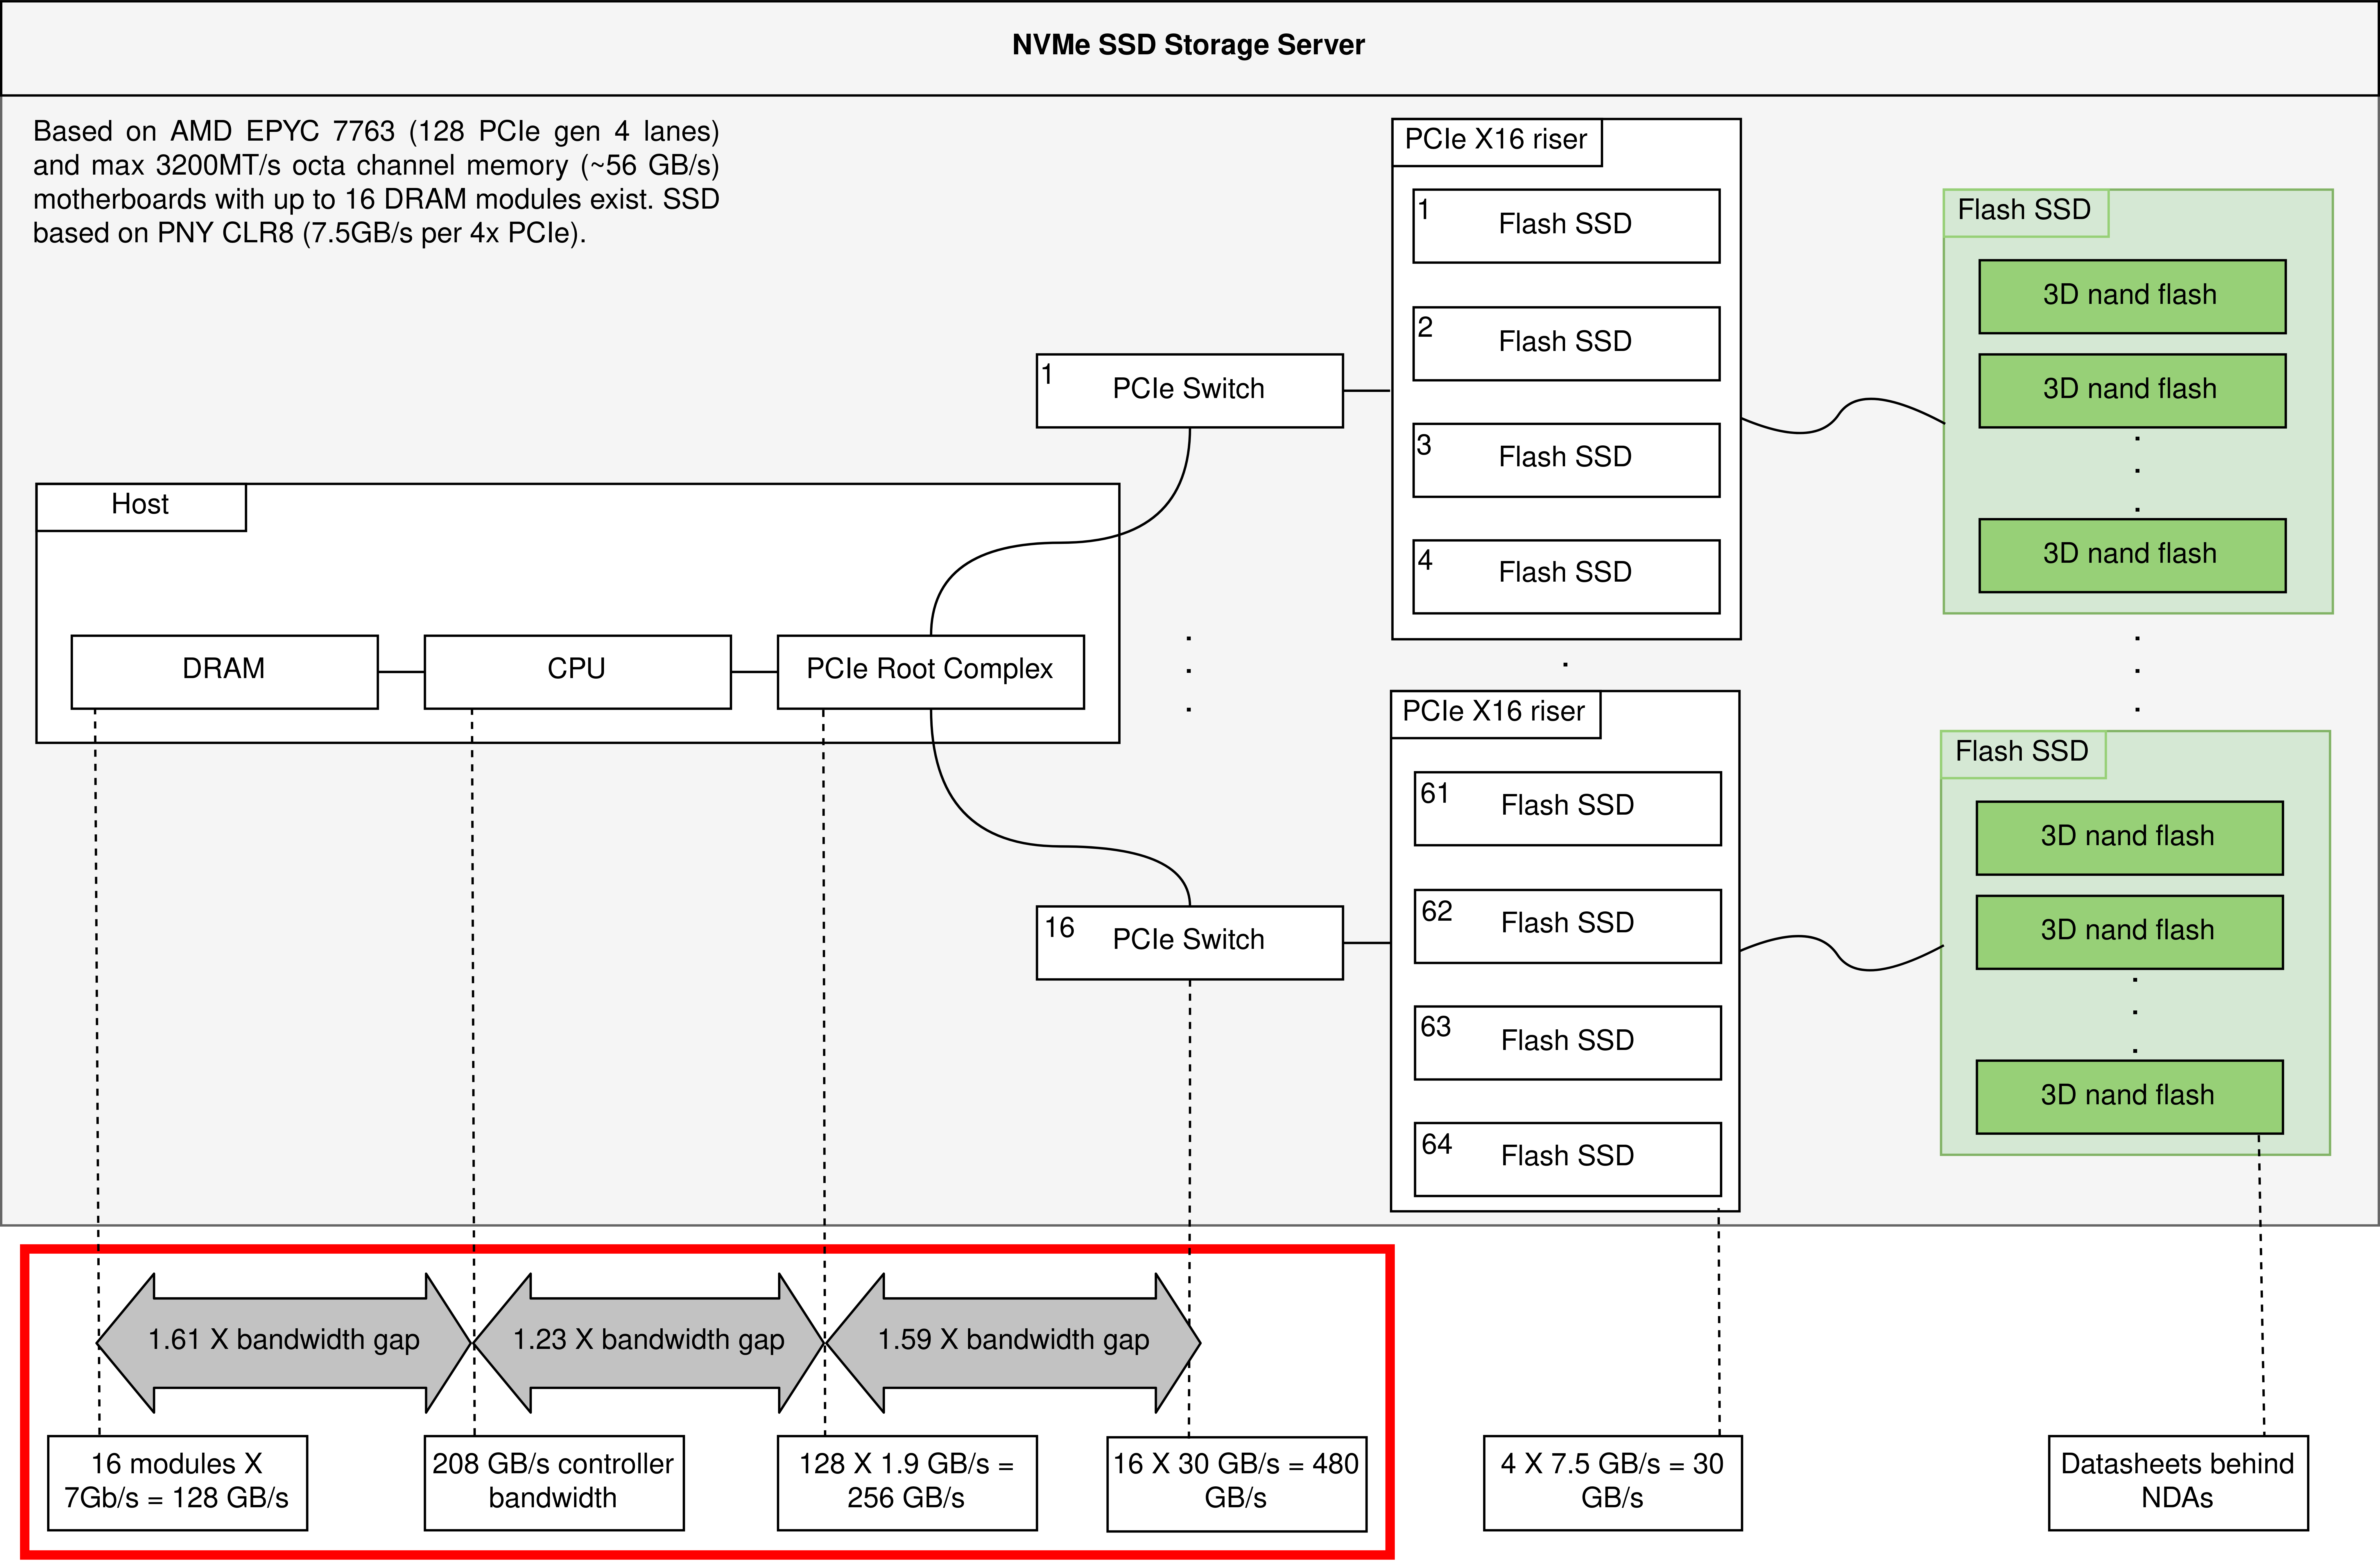
\includegraphics[width=0.8\textwidth]{resources/images/storage-bottleneck.png}
	\end{figure}
	\endgroup
\end{frame}

% page 3
\begin{frame}{Zoned NameSpaces (ZNS)}
	\begingroup
	\small
	\begin{itemize}
		 % nand flash needs to be linearly written while block interface allows arbitrary read / write and erase
		\item Better reflect Flash storage
		\item Block interface
		% To support this interface SSDs do a lot of internal translation
		\item The semantic gap
		% Expose a more natural interface of flash and make the host take care of translations
		\item host-managed
		\item Ratified extension [2]
		\item First commercial devices
	\end{itemize}
	\textit{\tiny $^{2}$NVM Express Zoned Namespace Command Set Specification 1.1b - 
	https://nvmexpress.org/developers/nvme-command-set-specifications/}
	\endgroup
\end{frame}

% page 4
\begin{frame}{Log-structured FileSystem (LFS)}
	\begingroup
	\small
	% Append only writes
	% Simple support for journaling, snapshotting and revovery
	% Our design based on F2FS to prevent write-amplification
	\begin{figure}
		\centering
		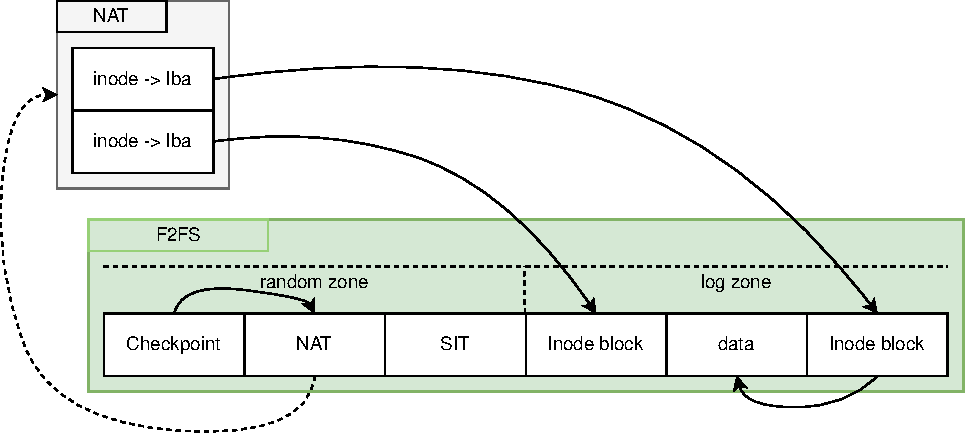
\includegraphics[width=0.7\textwidth]{resources/images/f2fs-nat.pdf}
	\end{figure}
	\textit{\tiny $^{3}$The design and implementation of a log-structured file system \\}
	\textit{\tiny $^{4}$F2FS: A New File System for Flash Storage}
	\endgroup
\end{frame}

% page 5
\begin{frame}{extended Berkely Packet Filter (eBPF)}
	\begingroup
	\small
	% used in the Linux kernel but effectively its an ISA like x86 but easy
	% to implement in virtual machines
	\begin{figure}
		\centering
		\includegraphics[width=0.7\textwidth]{resources/images/ubpf-abi.pdf}
	 \end{figure}
	\endgroup
\end{frame}

% page 6
\begin{frame}{OpenCSD}
	\begingroup
	\small Module based, simple to use \& install
	\begin{figure}
		\centering
		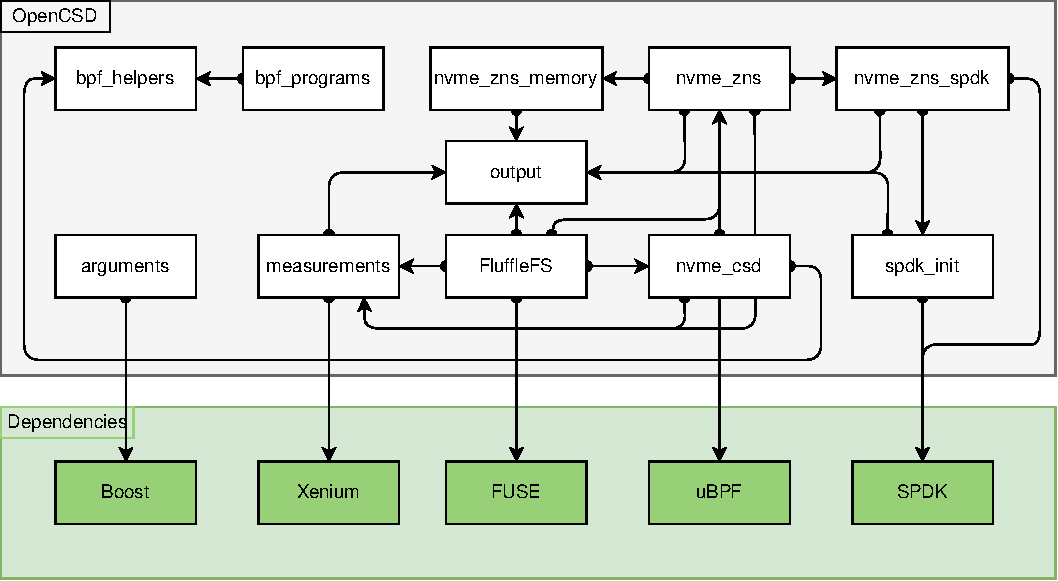
\includegraphics[width=0.8\textwidth]{resources/images/module-dependencies.pdf}
	\end{figure}
	\endgroup
\end{frame}

% page 7
\begin{frame}{FluffleFS}
	\begingroup
	% \small An emulated programmable computational flash storage device
	% \begin{figure}
	% 	\centering
	% 	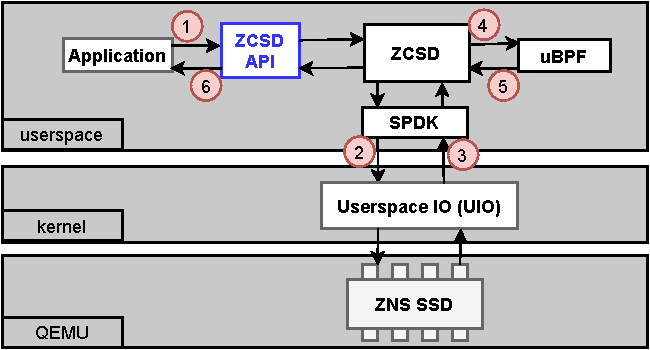
\includegraphics[width=0.8\textwidth]{resources/images/zcsd-arch-final}
	% \end{figure}
	\endgroup
\end{frame}

% page 8
\begin{frame}{Evaluation Microbenchmarks}
	\begingroup
	% \small An emulated programmable computational flash storage device
	% \begin{figure}
	% 	\centering
	% 	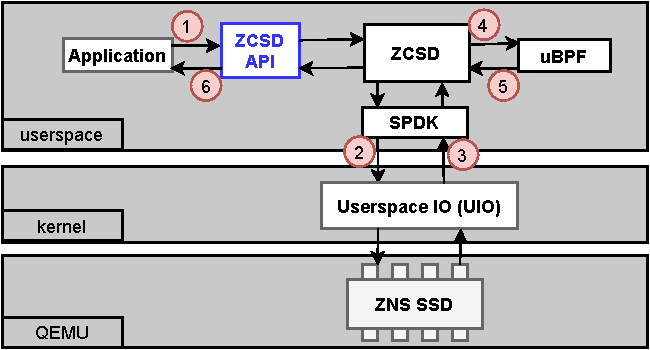
\includegraphics[width=0.8\textwidth]{resources/images/zcsd-arch-final}
	% \end{figure}
	\endgroup
\end{frame}

% page 9
\begin{frame}{Evaluation Application}
	\begingroup
	% \small An emulated programmable computational flash storage device
	% \begin{figure}
	% 	\centering
	% 	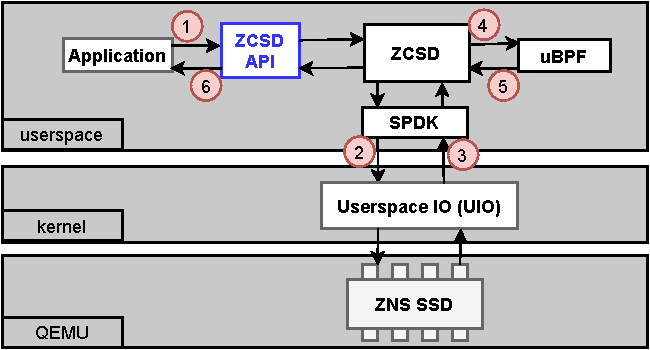
\includegraphics[width=0.8\textwidth]{resources/images/zcsd-arch-final}
	% \end{figure}
	\endgroup
\end{frame}

% page 10
\begin{frame}{Future Work}
	\begingroup
	\small Improve filesystem integration \& security
	\begin{figure}
		\centering
		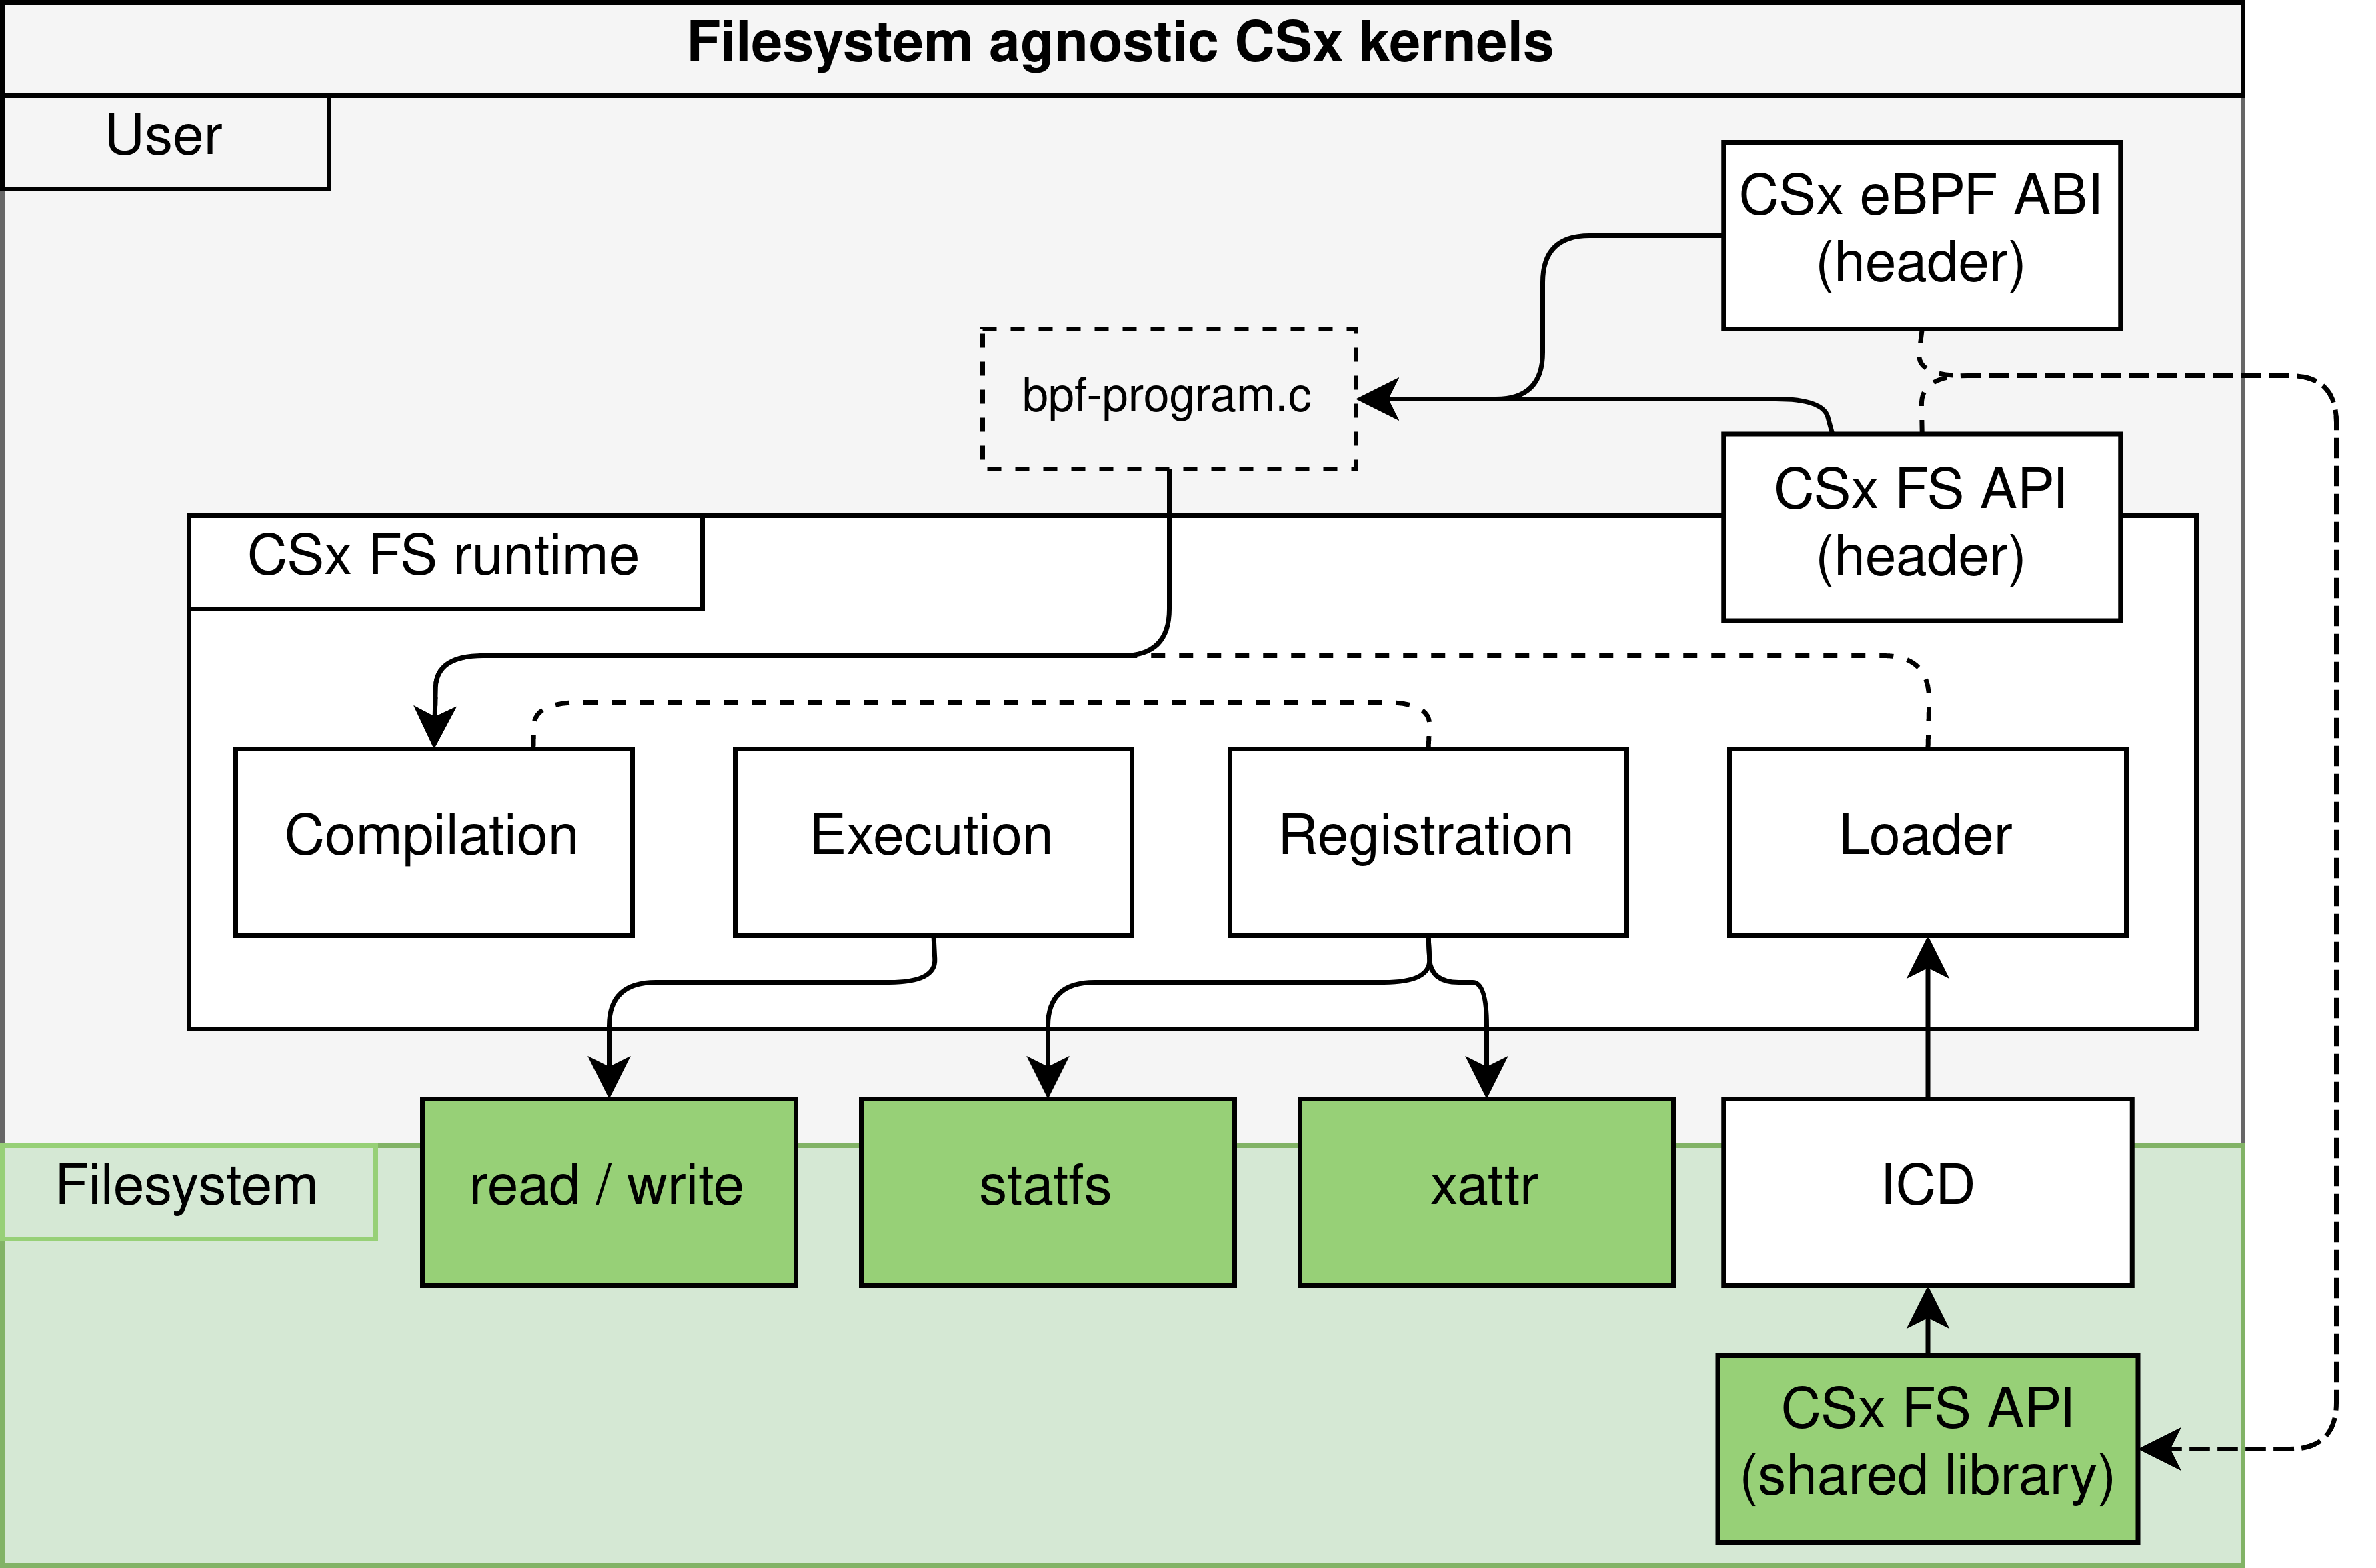
\includegraphics[width=0.8\textwidth]{resources/images/csx-fs-agnostic.png}
	\end{figure}
	\endgroup
\end{frame}

\end{document}